%!TEX encoding = UTF-8 Unicode
\documentclass[french]{article}
\usepackage{varwidth}
\usepackage{systeme}
\usepackage{breqn}


%% Langue et compilation

\usepackage[utf8]{inputenc}
\usepackage[T1]{fontenc}
\usepackage[french]{babel}

%% LISTE DES PACKAGES

\usepackage{mathtools}     % package de base pour les maths
\usepackage{amsmath}       % mathematical type-setting
\usepackage{amssymb}       % symbols speciaux pour les maths
\usepackage{textcomp}      % symboles speciaux pour el text
\usepackage{gensymb}       % commandes generiques \degree etc...
\usepackage{tikz}          % package graphique
\usepackage{wrapfig}       % pour entourer a cote d'une figure
\usepackage{color}         % package des couleurs
\usepackage{xcolor}        % autre package pour les couleurs
\usepackage{pgfplots}      % pacakge pour creer des graph
\usepackage{epsfig}        % permet d'inclure des graph en .eps
\usepackage{graphicx}      % arguments dans includegraphics
\usepackage{pdfpages}      % permet d'insérer des pages pdf dans le document
\usepackage{subfig}        % permet de creer des sous-figure
\usepackage{pst-all}       % utile pour certaines figures en pstricks
\usepackage{lipsum}        % package qui permet de faire des essais
\usepackage{array}         % permet de faire des tableaux
\usepackage{multicol}      % plusieurs colonnes sur une page
\usepackage{enumitem}      % pro­vides user con­trol: enumerate, itemize and description
\usepackage{hyperref}      % permet de creer des hyperliens dans le document
\usepackage{lscape}        % permet de mettre une page en mode paysage
\usepackage{lmodern}       % permet d'avoir certains "fonts" de bonen qualite
\usepackage{fancyhdr}      % Permet de mettre des informations en hau et en bas de page      
\usepackage[framemethod=tikz]{mdframed} % breakable frames and coloured boxes
\usepackage[left = 2cm, right = 2cm, top = 2.5cm, bottom = 2.5cm, landscape,twocolumn]{geometry}
\usepackage[font=normalsize, labelfont=bf,labelsep=endash, figurename=Fig.]{caption} % permet de changer les legendes des figures

%% LIBRAIRIES

\usetikzlibrary{plotmarks} % librairie pour les graphes
\usetikzlibrary{patterns}  % necessaire pour certaines choses predefinies sur tikz
\usetikzlibrary{shadows}   % ombres des encadres
\usetikzlibrary{backgrounds} % arriere plan des encadres
\usetikzlibrary{calc}
\usepackage{chngcntr}
\usetikzlibrary{backgrounds}
\usetikzlibrary{decorations.text}
\usetikzlibrary{decorations}
\usetikzlibrary{shapes.geometric}
\usetikzlibrary{decorations.pathreplacing}
\usetikzlibrary{calc}
\usetikzlibrary{%
    calc,%
    fadings,%
    shadings%
}
%% MISE EN PAGE

\pagestyle{fancy}     % Défini le style de la page

\renewcommand{\headrulewidth}{1pt}      % largeur du trait en haut de la page
\fancyhead[L]{Montage de Physique}         % info coin haut gauche
\fancyhead[R]{Université de Rennes 1}  % info coin haut droit

% bas de la page
\renewcommand{\footrulewidth}{1pt}      % largeur du trait en bas de la page
\fancyfoot[L]{Gabriel \bsc{LE DOUDIC}}  % info coin bas gauche
\fancyfoot[R]{Préparation à l'Agrégation de Physique}                         % info coin bas droit


\setlength{\columnseprule}{1pt} 
\setlength{\columnsep}{30pt}



%% NOUVELLES COMMANDES 

\DeclareMathOperator{\e}{e} % permet d'ecrire l'exponentielle usuellement


\newcommand{\gap}{\vspace{0.15cm}}   % defini une commande pour sauter des lignes
\renewcommand{\vec}{\overrightarrow} % permet d'avoir une fleche qui recouvre tout le vecteur
\newcommand{\bi}{\begin{itemize}}    % begin itemize
\newcommand{\ei}{\end{itemize}}      % end itemize
\newcommand{\bc}{\begin{center}}     % begin center
\newcommand{\ec}{\end{center}}       % end center
\newcommand\opacity{1}               % opacity 
\pgfsetfillopacity{\opacity}

\newcommand*\Laplace{\mathop{}\!\mathbin\bigtriangleup} % symbole de Laplace

\frenchbsetup{StandardItemLabels=true} % je ne sais plus

\newcommand{\smallO}[1]{\ensuremath{\mathop{}\mathopen{}o\mathopen{}\left(#1\right)}} % petit o

\newcommand{\cit}{\color{blue}\cite} % permet d'avoir les citations de couleur bleues
\newcommand{\bib}{\color{black}\bibitem} % paragraphe biblio en noir et blanc
\newcommand{\bthebiblio}{\color{black} \begin{thebibliography}} % idem necessaire sinon bug a cause de la couleur
\newcommand{\ethebiblio}{\color{black} \end{thebibliography}}   % idem
%%% TIKZ


%% COULEURS 


\definecolor{definitionf}{RGB}{220,252,220}
\definecolor{definitionl}{RGB}{39,123,69}
\definecolor{definitiono}{RGB}{72,148,101}

\definecolor{propositionf}{RGB}{255,216,218}
\definecolor{propositionl}{RGB}{38,38,38}
\definecolor{propositiono}{RGB}{109,109,109}

\definecolor{theof}{RGB}{255,216,218}
\definecolor{theol}{RGB}{160,0,4}
\definecolor{theoo}{RGB}{221,65,100}

\definecolor{avertl}{RGB}{163,92,0}
\definecolor{averto}{RGB}{255,144,0}

\definecolor{histf}{RGB}{241,238,193}

\definecolor{metf}{RGB}{220,230,240}
\definecolor{metl}{RGB}{56,110,165}
\definecolor{meto}{RGB}{109,109,109}


\definecolor{remf}{RGB}{230,240,250}
\definecolor{remo}{RGB}{150,150,150}

\definecolor{exef}{RGB}{240,240,240}

\definecolor{protf}{RGB}{247,228,255}
\definecolor{protl}{RGB}{105,0,203}
\definecolor{proto}{RGB}{174,88,255}

\definecolor{grid}{RGB}{180,180,180}

\definecolor{titref}{RGB}{230,230,230}

\definecolor{vert}{RGB}{23,200,23}

\definecolor{violet}{RGB}{180,0,200}

\definecolor{copper}{RGB}{217, 144, 88}

%% Couleur des ref

\hypersetup{
	colorlinks=true,
	linkcolor=black,
	citecolor=blue,
	urlcolor=black
		   }

%% CADRES


%%%%%%%%%% DEFINITION

\newmdenv[tikzsetting={fill=definitionf}, linewidth=2pt, linecolor=definitionl, outerlinewidth=0pt, innertopmargin=5pt, innerbottommargin=5pt, innerleftmargin=5pt, innerrightmargin=5pt, leftmargin=0pt]{definition}

\newmdenv[ tikzsetting={drop shadow={ shadow xshift=1ex, shadow yshift=-0.5em, fill=definitiono, opacity=1, every shadow } }, outerlinewidth=2pt, outerlinecolor=white, linecolor=white, innertopmargin=0pt, innerbottommargin=0pt, innerleftmargin=0pt, innerrightmargin=0pt]{ombredef}


%%%%%%%%%% THEOREME

\newmdenv[tikzsetting={fill=theof}, linewidth=2pt, linecolor=theol, outerlinewidth=0pt, innertopmargin=5pt, innerbottommargin=5pt, innerleftmargin=5pt, innerrightmargin=5pt, leftmargin=0pt]{theo}

\newmdenv[ tikzsetting={drop shadow={ shadow xshift=1ex, shadow yshift=-0.5em, fill=theoo, opacity=1, every shadow } }, outerlinewidth=2pt, outerlinecolor=white, linecolor=white, innertopmargin=0pt, innerbottommargin=0pt, innerleftmargin=0pt, innerrightmargin=0pt]{ombretheo}


%%%%%%%%%% METHODE

\newmdenv[tikzsetting={fill=metf}, linewidth=2pt, linecolor=metl, outerlinewidth=0pt, innertopmargin=5pt, innerbottommargin=5pt, innerleftmargin=5pt, innerrightmargin=5pt, leftmargin=0pt]{met}

\newmdenv[ tikzsetting={drop shadow={ shadow xshift=1ex, shadow yshift=-0.5em, fill=meto, opacity=1, every shadow } }, outerlinewidth=2pt, outerlinecolor=white, linecolor=white, innertopmargin=0pt, innerbottommargin=0pt, innerleftmargin=0pt, innerrightmargin=0pt]{ombremet}



%%%%%%%%%%% RQ

\newmdenv[tikzsetting={fill=remf}, linewidth=2pt, linecolor=remf, outerlinewidth=0pt, innertopmargin=5pt, innerbottommargin=5pt, innerleftmargin=5pt, innerrightmargin=5pt, leftmargin=0pt]{remarque}

\newmdenv[ tikzsetting={drop shadow={ shadow xshift=1ex, shadow yshift=-0.5em, fill=remo, opacity=1, every shadow } }, outerlinewidth=2pt, outerlinecolor=white, linecolor=white, innertopmargin=0pt, innerbottommargin=0pt, innerleftmargin=0pt, innerrightmargin=0pt]{ombreremarque}

%%%%%%%%%%% Cadre pour le titre
\mdfsetup{ roundcorner=10pt}

\tikzset{every shadow/.style={opacity=1}}

\global\mdfdefinestyle{doc}{backgroundcolor=white, shadow=true, shadowcolor=propositiono, linewidth=1pt, linecolor=black, shadowsize=5pt}
\global\mdfdefinestyle{titr}{backgroundcolor=metf, shadow=true, shadowcolor=propositiono, linewidth=1pt, linecolor=black, shadowsize=5pt}

\global\mdfdefinestyle{theo}{backgroundcolor=theof, shadow=true, shadowcolor=theoo, linewidth=1pt, linecolor=theol, shadowsize=5pt}

\global\mdfdefinestyle{prop}{backgroundcolor=theof, shadow=true, shadowcolor=propositiono, linewidth=1pt, linecolor=theol, shadowsize=5pt}
\global\mdfdefinestyle{def}{backgroundcolor=definitionf, shadow=true, shadowcolor=definitiono, linewidth=1pt, linecolor=definitionl, shadowsize=5pt}
\global\mdfdefinestyle{histo}{backgroundcolor=histf, shadow=true, shadowcolor=propositiono, linewidth=1pt, linecolor=black, shadowsize=5pt}
\global\mdfdefinestyle{avert}{backgroundcolor=white, shadow=true, shadowcolor=averto, linewidth=1pt, linecolor=avertl, shadowsize=5pt}
\global\mdfdefinestyle{met}{backgroundcolor=metf, shadow=true, shadowcolor=meto, linewidth=1pt, linecolor=metl, shadowsize=5pt}

\global\mdfdefinestyle{rem}{backgroundcolor=metf, shadow=true, shadowcolor=meto, linewidth=1pt, linecolor=metf, shadowsize=5pt}

\global\mdfdefinestyle{exo}{backgroundcolor=exef, shadow=true, shadowcolor=propositiono, linewidth=1pt, linecolor=exef, shadowsize=5pt}
\global\mdfdefinestyle{not}{backgroundcolor=definitionf, shadow=true, shadowcolor=propositiono, linewidth=1pt, linecolor=black, shadowsize=5pt}
\global\mdfdefinestyle{proto}{backgroundcolor=protf, shadow=true, shadowcolor=proto, linewidth=1pt, linecolor=protl, shadowsize=5pt}


%%%%%%



\def\width{12}
\def\hauteur{5}

\setlength{\parskip}{0pt}%
\setlength{\parindent}{18pt}


%% MODIFICATION DE CHAPTER  
\makeatletter
\def\@makechapterhead#1{%
  %%%%\vspace*{50\p@}% %%% removed!
  {\parindent \z@ \raggedright \normalfont
    \ifnum \c@secnumdepth >\m@ne
        \huge\bfseries \@chapapp\space \thechapter
        \par\nobreak
        \vskip 20\p@
    \fi
    \interlinepenalty\@M
    \Huge \bfseries #1\par\nobreak
    \vskip 40\p@
  }}
\def\@makeschapterhead#1{%
  %%%%%\vspace*{50\p@}% %%% removed!
  {\parindent \z@ \raggedright
    \normalfont
    \interlinepenalty\@M
    \Huge \bfseries  #1\par\nobreak
    \vskip 40\p@
  }}
\makeatother

\usepackage{dashundergaps}
\newcommand{\croix}[2]{\draw[very thick] (#1,#2-0.15)-- (#1,#2+0.15);\draw (#1-0.15,#2)-- (#1+0.15,#2);}

\global\mdfdefinestyle{rem}{backgroundcolor=metf, shadow=true, shadowcolor=meto, linewidth=1pt, linecolor=metf, shadowsize=5pt}

%%
%% DEBUT DU DOCUMENT
%%

\begin{document}
\tikzset{every shadow/.style={opacity=1}}


\begin{center}
	\begin{mdframed}[style=titr, leftmargin=55pt, rightmargin=55pt, innertopmargin=8pt, innerbottommargin=8pt, innerrightmargin=10pt, innerleftmargin=10pt]
		
		
		\begin{center}
			\large{\textbf{Montage de Physique}} \\
			\Large{\textbf{Interférences lumineuses}}
		\end{center}
		
	\end{mdframed}
\end{center}

\noindent\textbf{\large Références:}\gap

\begin{itemize}
	\item Poly TP de Rennes;
	\item Poly de TP Montrouge;
	\item Sextant. Optique experimentale;
	\item Bertin Faroux Renaut. Optique et physique ondulatoire.
	\item Sylvain Houard. Optique, une approche expérimentale et pratique;
\end{itemize}

\section{Fentes d'Young}

Lorsqu'on éclaire un dispositif interférentiel  avec une source ponctuelle (cohérence spatiale parfaite) et monochromatique (cohérence temporelle parfaite). On obtient des interférences avec un contraste maximum et sensiblement constant dans tout l'espace de superposition des ondes.\vspace{.15cm}

Il faut des bi-fentes suffisamment fines pour avoir une figure de diffraction large et suffisamment proches pour obtenir un interfrange appréciable. L'importance historique de ce montage est grande car il a permis pour la première fois d'évaluer des longueurs d'ondes lumineuses. 


\subsection{Principe et schéma}

On considère une source S de très petite dimension (laser He-Ne) éclaire un écran opaque percé de deux fentes dont les dimensions sont très faibles. D'après les lois de l'optique géométrique on devrait obtenir sur cet écran les traces de M1 et M2 des deux raions SS1 et SS2. Cependant la diffraction intervient du fait des faibles dimensions de S1 et S2 et l'on obtient des faiscequx qui se recouvrent. C'est dans cette zone que l'on peut observer des interférences appelée \textbf{zone interférencielle}. 

S1 et S2 sont des sources \textbf{cohérentes dont les rayons interfèrent} et de même intensité I0. Dans le plan de l'écran, on obtient une intensité donnée par : 
\begin{definition}
\begin{equation}
	I = 2I_0\left(1+\cos\phi\right), \text{ avec } \phi = \frac{2\pi\delta}{\lambda} = \frac{2\pi}{\lambda}\left(S_2M-S_1M\right). 
\end{equation}
\end{definition}
On peut calculer la différence de marche entre les deux sources $\delta$ qui est donnée par : 

\begin{equation}
	\delta = \frac{ax}{d_2}
\end{equation}

$x$ étant la position verticale sur l'écran. Les franges obtenues sont donc des franges d'interférences rectilignes parallèles à $Oy$ (perpendiculaire à la direction de $S_1S_2$).
\begin{figure}[!ht]
	\centering
	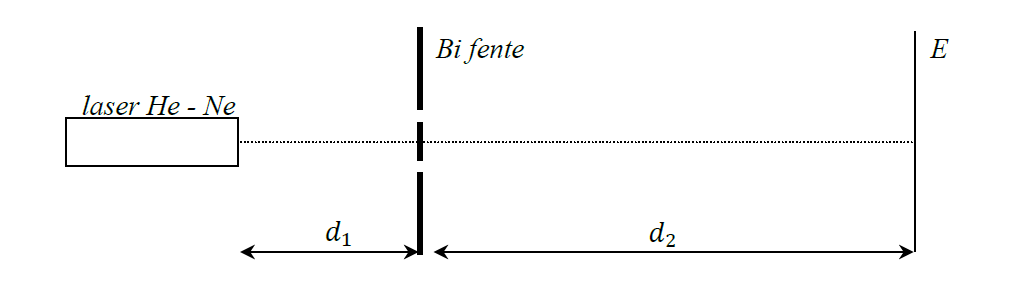
\includegraphics[width = .5\textwidth]{./figures/Bifente_DYoung.png}
	\caption{Schéma de principe des fentes d'Young}
\end{figure}

\begin{remarque}
	\begin{itemize}
		\item Laser He-Ne $\lambda = 632.8$ nm;
		\item Écartement des fentes $a = 0.6$ mm;
		\item Largeur des fentes $b = 0.12$ mm.
	\end{itemize}
\end{remarque}

\subsection{Observation}
\subsubsection{Allure de la figure d'interférence}

Dans ce cas où la fente est éclairée par une source de lumière monochromatique $\lambda_0$. Pour $\delta = p\lambda_0$ on obtient des franges prillantes. Leur position est définie pour $\frac{ax}{d_2}=p\lambda$ soit : 
$$x = p\left(\frac{\lambda_0d_2}{a}\right)$$

Pour $p=0$ et $x=0$ on a une frange brillante centrale qui correspond à un ordre d'interférence nul. Les franges brillantes sont séparées par une intervalle régulière : 
\begin{equation}
	i = \frac{\lambda_0d_2}{a}
\end{equation}
\subsubsection{Mesure de l'écartement des fentes}
\begin{remarque}
	\begin{itemize}
		\item Interfrange $i = $ \gap*[-]{texte texte} $\pm$ \gap*[-]{texte texte} mm
		\item Distance fentes-écran $d_2 = $\gap*[-]{texte texte} $\pm$ \gap*[-]{texte texte} mm
	\end{itemize}
\end{remarque}

On calcule $$\lambda = \frac{ia}{d_2}$$

\begin{theo}
	\textbf{Mesure de l'écartement des deux fentes:}\gap 

	$\lambda_{\rm mes} = $\gap*[-]{texte texte} $\pm$ \gap*[-]{texte texte} nm
\end{theo}

\noindent \textbf{Écart normalisé:}
\[E.N. = \frac{\lambda_{\rm mes}- \lambda_{\rm att}}{\sqrt(\Delta \lambda_{\rm mes}^2+\Delta \lambda_{\rm att}^2 )} = \text{\gap*[--]{text text}}\]


\noindent\textbf{Conclusion:}\gap

On notera que la position de l'écran est quelconque. On dit que les interférences obtenues avec ce dispositif sont  \textbf{non localisées}. Cela fonctionne, car nous travaillons avec une source ponctuelle.\vspace{.5cm}

\noindent\textbf{Quid de la lumière blanche:}\gap 

Si la source est une lumière blanche. On obtient dans le plan de l'écran une superposition de phénomènes correspondants aux différentes longueur d'ondes. On obtient alors des phénomènes colorés. Au centre une frange brillante achromatique. Quand on s'éloigne du centre, les phénomènes correspondants aux différentes longeurs d'onde se décalent de plus en plus: les bords des franges se colorent puis les phénomènes se brouillent lorsques les franges brillantes d'autres longeurs d'onde occupent la même place. On obtient du \textbf{blanc d'ordre supérieur}. L'interféromètre des fentes d'Young se prète mal aux expériences en lumière blanche mais est facile à réaliser avec l'interféromètre de Michelson.

\section{Interféromètre de Michelson}
Le Michelson en anneaux est moins sensible à la cohérence spatiale de la source si on observe les interférences au loin. Il est en toute rigueur complètement insensible à la cohérence spatiale lorsque l'on effectue une observation à l'infini (observation dans le plan focal image d'une lentille). Cette propriété est très importante en spectroscopie car elle permet d'étudier les problèmes de cohérence temporelle d'une source indépendamment de sa cohérence spatiale. 

\subsection{Principe et schéma}

Un interféromètre est constitué d'une lame semi-réfléchissante non-absorbante appelée séparatrice ($S_p$) (les facteurs de transmission et de réflexion valent 1/2), d'une compensatrice et de deux miroirs plans $M_1$ et $M_2$ perpendiculaires l'un par rapport à l'autre. La lame $S_p$ est inclinée de $45^{\circ}$ par rapport aux normales des deux miroirs.\gap


Lorsqu’un rayon arrive sur la séparatrice, il est séparé en deux. Les deux « parties » du rayon se réfléchissent sur M1 ou $M_2$, et sont réfléchis (ou transmis) vers l’axe sortant du dispositif par la sépa-ratrice. La compensatrice assure une égalité des chemins optiques des deux voies de l’interféromètre.\gap

Lorsque les deux miroirs dont équidistants de la séparatrice  et symétriques par rapport à la séparatrice, on dit que l'interféromètre est configuré en lame d'air et la différence de marche entre les deux rayons est donnée par: 

\begin{equation}
	\delta = 2e\cos{\theta}.
\end{equation}

$e$ étant la différence de distance entre les deux miroirs par rapport à la séparatrice. $\theta$ est l'angle d'incidence entre l'axeoptique et la séparatrice.

\begin{figure}[!ht] 
	\centering
	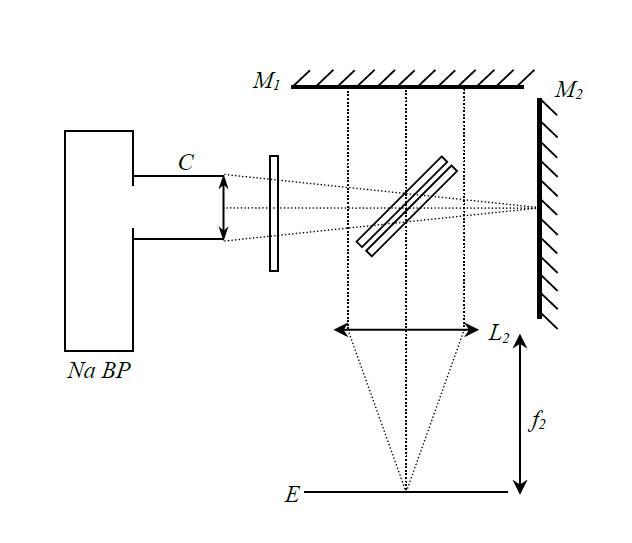
\includegraphics[width=.3\textwidth]{./figures/MichelsonLameDair.png}
	\caption{Inteféromètre de Michelson réglé en lame d'air.}
\end{figure}

\begin{remarque}
	\begin{itemize}
		\item Condenseur C de 6 cm.
		\item Lentille $L2$, $f'= 50~\rm cm$.
		\item Lampe à vapeur de sodium $\lambda = 589.3$ nnm.
		\item distance entre raies $\Delta\lambda = 0.6$ nm.
	\end{itemize}
\end{remarque}

\subsubsection{Réglage}

Voir annexe
\subsection{Observations}

\subsubsection{Allure de la figure d'interférence}

Lorsque l’interféromètre sera configuré en lame d’air, on observera des anneaux concentriques,
ou « franges d’égale inclinaison ». On observe les anneaux d'intensité maximale lorsque $\theta$ vérifie $$cos(\theta) = p
\frac{\lambda}{2e}$$ avec $p\in \mathbb{N}$. Les franges d’égales inclinaison sont localisées à l’infini devant M1. Il y a donc deux manières (physiquement équivalentes) de les observer : En observant M1 à l’œil nu. En effet, le cristallin projettera les franges sur la rétine. On peut également les observer avec une caméra munie de son objectif. Ou en plaçant une lentille convergente en sortie de l’interféromètre, et un écran dans le plan focal image de cette lentille. La figure d’interférence sera alors projetée sur l’écran.

\subsubsection{Mesure du doublet du sodium}
On cherche à étudier l'influence de l'étendue spectrale d'une source sur le contraste de la figure d'interférences que peut fournir un dispositif interférentiel. On suppose qu'il n'y a pas de problème de cohérence spatiale.\vspace{.5cm}

Deux ondes monochromatiques de fréquence très légèrement différentes ne peuvent interférer de façon cohérente à l'échelle des temps de réponse caractéristique des détecteurs optiques car la différence de phase varie trop rapidement. Elles sont dites temporellement incohérentes entres elles. Ce problème intervient toujours avec une source réelle puisqu'elle émet dans un spectre plus ou moins étendu. Pour comprendre ce résultat il suffit de la considérer comme une collection de raies élémentaires, quasi monochromatiques et incohérentes entre elles. Chaque raie contribue à la figure d'interférence par une figure élémentaire dont l'interfrange dépend de la longuer d'onde. Chaque figure élémentaire s'ajoute aux autres en intensité et affaiblit ainsi le contraste de la figure totale.\vspace{.15cm}

L'emploi du Michelson est une méthode de choix pour faire des études spectrales de sources étendues car il est insensible à la cohérence spatiale quand on observe à l'infini.
\vspace{.15cm}

Lorsqu'on chariote de part et d'autre du contact optique, on s'aperçoit que le contraste est modulé en fonction de $\delta$ et s'annule périodiquement pour un chariotage $\Delta e \approx 0.3$ mm. Le sodium est principalement constitué d'une raie jaune $\lambda = 589.3$ nm qui est en fait un doublet de raies fines distantes de $\Delta \lambda$.

Pour passer d’un brouillage à l’autre, la longueur d’onde $\lambda_1$ la plus courte du doublet a subi une variation de différence de marche égale à $\left(p+1\right)\lambda_1$ alors que la longueur d’onde $\lambda_2$ la plus grande a subi une variation de différence de marche de $p\lambda_2$. Sur le trajet optique du Michelson cela correspond $2\Delta e_1$.

\[\Delta \lambda = \frac{\lambda^2}{2\Delta e_1} = \frac{n\lambda ^2}{2\Delta e_n}\]

\noindent avec $\lambda = \lambda_1 = \lambda_2$ et $\Delta\lambda  = \lambda_2 - \lambda_1$.

Pour mesurer $\Delta \lambda$ on chariote pour passer d'un brouillage à l'autre. On relève $\Delta e$ parcourue par le chariot pour passer d'un brouillage au n-ième suivant. 

\begin{remarque}
	\begin{itemize}
		\item Distance parcourue $\Delta e = $ \gap*[-]{texte texte} $\pm$ \gap*[-]{texte texte} mm
	\end{itemize}
\end{remarque}


On peut aussi relever la position des différentes annulations $e_k$ et les tracer en fonction de $k$. Médliser par une droite affine $e_k = ak + b$. Interpréter $a$ et la moyenne quadratique des écarts.

\begin{theo}
	\textbf{Mesure du doublet du sodium:}\vspace{.5cm}

	\[\Delta \lambda_{\rm mes} = \text{\gap*[-]{text text}} \pm \text{\gap*[-]{text text}} \text{ nm}\]
\end{theo}

\[E.N. = \frac{\lambda_{\rm mes}- \lambda_{\rm att}}{\sqrt(\Delta \lambda_{\rm mes}^2+\Delta \lambda_{\rm att}^2 )} = \text{\gap*[--]{text text}}\]


\noindent \textbf{Élargissement:}\vspace{.5cm}

Les franges d'égales épaisseur, obtenues à l'aide de l'interféromètre de Michelson réglé en coin d'air, s'observent couramment dans la nature sous forme d'irisation à la surface de bulles de savon ou de flaques recouvertes d'une pellicule huileuse. Un simple film de savon tendu sur un cadre permet de réaliser des expériences spectaculaires avec un appareil réduit.

\section{Polarisation des ondes}

\subsection{Principe}

Certains matériaux présentent une anisotropie optique liée à une anisotropie de structure. Dans ce type de composés, la biréfringence se manifeste par un comportement optique différent suivant l'orientation du champ électrique de la vibration lumineuse. Si on se limite aux milieux uniaxes on peut montrer que la vibration lumineuse incidente se décompose en 2 vibration rectilignes orientées suivant les 2 lignes neutres du cristal qui se propagent avec des vitesses différentes. À la sortie de la lame elles ont donc un déphasage:
\begin{equation}
	\phi = \frac{2\pi\delta}{\lambda} = \frac{2\pi(n_e'-n_0)e}{\lambda}
\end{equation}

et peuvent interférer. Pour ce faire il faut une lumière polarisée et un analyseur pour recomposer les vibrations.

\begin{figure}
	\centering
	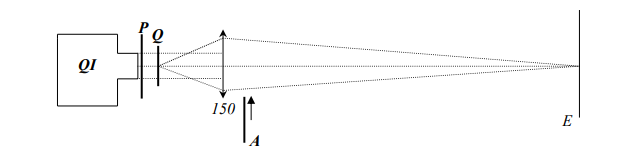
\includegraphics[width = .5\textwidth]{./figures/Polarisation.png}
	\caption{Montage: polarisation des ondes}
\end{figure}

\begin{figure}
	\centering
	\includegraphics[width=.5\textwidth]{./figures/Finpolarisation.png}
\end{figure}
\newpage
\section{Épaisseur d'un film de savon}

\subsection{Principe et schéma}
Les couches minces naturelles telles que les films d'eau savonneux ou d'huile sur la chaussée détrempée ne possèdent pas une épaisseur constante. Elles produisent des figures d'interférence formées de franges colorées dont la couleur dépend de l'épaisseur locale de la lame.\vspace{.5cm}


Pour former un film de savon on plonge un cadre metallique dans un melange d'eau, de liquide vaisselle transparent et de glycérine. On le retire et on le met à la verticale. On obtient alors un film dont la durée de vie peut atteindre plusieurs minutes.

\begin{figure}[!ht]
	\centering
	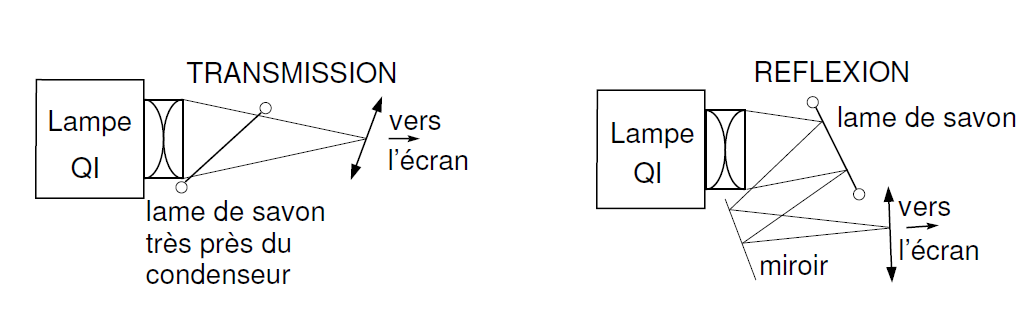
\includegraphics[width = .5\textwidth]{./figures/Filmsavon.png}
	\caption{Schéma du montage pour mesure de l'épaisseur d'un film de savon.}
\end{figure}


\begin{remarque}
	\begin{itemize}
		\item Liquide vaisselle transparent + glycérine
		\item cadre
		\item lampe QI
		\item miroir
	\end{itemize}
\end{remarque}


Dans le cas des franges constructives, on peut montrer que l'épaisseur du film $e$ est donnée par la relation: 

\begin{equation}
	e = \frac{\left(m-\frac{1}{2}\right)\lambda_0}{2n_s}
\end{equation}
La condition d'interérence constructive donne pour $m_1 = 1$: $e_1  = \frac{\lambda_0}{4n_2}$. $n_2$ est l'indice optique dans le savon et vaut $n_2 = 1.34$. Dans le visible $\lambda_0 \in [380, 760]$ nm. On obtient une plage d'épaisseur $e\in[71, 142]$ nm. Les premières interférences constructives se produiront pour une épaisseur de $71 nm$ pour des radiations violettes. On aura une épaisseur maximale de $e=142$ nm pour des radiations rouges.

Dans le cas des interférences destructives, on peut montre que $e$ est donnée par : 

\begin{equation}
	e = \frac{m\lambda_0}{2n_s}.
\end{equation}

La condition d’inteférence destructive est donnée par $m_2 = 1$, $e_2 = \frac{λ_0}{2n_s}$. On obtient une plage e ∈ [142, 284] nm.


\subsubsection{Observations}

\subsubsection{Allure de la figure d'interférence}

\begin{wrapfigure}{l}[10]{.2\textwidth}
	\begin{tikzpicture}[scale = 2.5]
		\draw (0,0) -- (2,0)--(2,2) -- (0,2) --cycle;
		\draw (1,1) node{Ajouter photo des interférences};
	\end{tikzpicture}
	\caption{Figure d'interférence}
\end{wrapfigure}
On peut observer trois stades: 
\begin{enumerate}
	\item Dans un premier temps, l'épaisseur du film est trop importante et aucune frange colorée n'apparaît.
	\item La gravité entraîne du liquide vers le bas. L'amincissement du film en haut, permet l'apparition de frange de couleur rose. Le drainage se poursuit, des franges roses et vertes alternées apparaîssent dans la partie supérieur. Puis de nouvelles franges colorées, très vives, apparaissent.
	\item Juste avant son éclatement, le film présente une raie blanchâtre à son sommet, voir même une frange non réfléchissante, lorsque $e$ ne mesure que quelques nm.
\end{enumerate}

\subsubsection{Mesure de l'épaisseur du film de savon}

\begin{remarque}
	\begin{itemize}
		\item $m = 1$ $\lambda_{0} = $ \gap*[-]{text text} $\pm$
 \gap*[-]{text text}
 	\item $m = 3$ $\lambda_{0} = $ \gap*[-]{text text} $\pm$
 \gap*[-]{text text}
 	\item $m = 5$ $\lambda_{0} = $ \gap*[-]{text text} $\pm$
 \gap*[-]{text text}	
	\end{itemize}
\end{remarque}


\begin{theo}
	\textbf{Mesures:}\vspace{.5cm}
	\begin{itemize}
		\item $e_1 =$ \gap*[-]{text text} $\pm$
		\gap*[-]{text text}
		\item $e_2 =$ \gap*[-]{text text} $\pm$
		\gap*[-]{text text}
		\item $e_3 =$ \gap*[-]{text text} $\pm$
		\gap*[-]{text text}
	\end{itemize}
\end{theo}

\section{Annexe 1. Réglage du Michelson}


On commence avant tout par bien positionner l’interféromètre sur la table. On effectue ensuite quelques ajustements, comme le réglage grossier 1 des miroirs (orientation et distance à la séparatrice), avant de s’assurer que toutes les vis sont approximativement à mi-course (ce qui nous permettra d’avoir une amplitude de réglage optimale par la suite).\vspace{.5cm}

À l’aide d’un collimateur, on règle le couple séparatrice-compensatrice, en s’assurant que séparatrice et compensatrice soient bien coplanaires. On cherchera pour cela à superposer l’image du réticule et ses diverses réflexions.
De la même façon, on règle approximativement l’orthogonalité des miroirs.\vspace{.5cm}

On cherche maintenant à visualiser les interférences, puis à trouver le contact optique. On effectuera d’abord un réglage grossier avec la lampe à Mercure, puis un réglage fin en lumière blanche.\vspace{.5cm}

On commence par éclairer l’interféromètre avec une lampe à vapeur de Mercure. En translatant légèrement M2, on voit apparaître des franges rectilignes, comme celles présentées
en Figure 1.3. On ajuste ensuite l’inclinaison des miroirs jusqu’à voir les franges rectilignes se
courber, puis former des anneaux. Une fois ces anneaux obtenus, on translate M2 pour avoir de moins en moins d’anneaux sur la
figure, jusqu’à observer une teinte presque uniforme, que l’on ajuste à l’aide des vis d’inclinaison micrométriques des miroirs. On a alors un contact optique approximatif.\vspace{.5cm}

En vue d’affiner le contact optique, on éclaire maintenant le dispositif en lumière blanche. On observe une figure d’interférence plus colorée, et on remarque que les réglages de l’interféromètre deviennent plus sensibles (une même modification de l’un des réglages semble affecter davantage la
figure d’interférence en lumière blanche que celle en lampe à Mercure). On comprend ainsi que le contact optique obtenu avec la lampe à Mercure n’était que très approximatif. On recherche de la même façon que précédemment le contact optique. On s’attend à voir des blancs d’ordres supérieurs (voir plus bas) si on en est éloigné, des franges colorées si l’on en est proche, et une lumière blanche uniforme s’il est atteint. On note alors, afin de le retrouver facilement, la position de la vis V1 : elle est à environ $V_1  = $ \gap*[-]{text text}.\vspace{.5cm}


Au contact optique, la différence de marche entre les deux voies de l’interféromètre est nulle. L’interféromètre est dit au « contact optique » lorsque M1 et M2 sont confondus. Ceci correspond au cas de la lame d’air avec $e = 0$. On s’attend dont à voir, en sortie de l’interféromètre, la lumière de la source sans aucune interférence. Partant du contact optique, on chariote  jusqu'à dépasser la première anti-coïncidence et retrouver des anneaux contrastés. On déplace alors l'écran de part et d'autre du foyer de la lentille $L_2$ et les franges devraient se brouiller. Le contraste est maximum lorsque l'écran est au foyer image de la lentille. On peut aussi observer les franges sans lentille en éloignant suffisamment l'écran.


\section{Annexe 2. Films de savon}

\subsection{Préparation du savon}

8 volumes d'eau (distillée), 1 volume de glycerine, 1 volume de liquide vaisselle.

\subsection{Théorie}
Pour simplifier on supposera que les rayons incidents arrivent sur la lame de savon sous incidence normale $\theta = 0$. Dans ces conditions, le trajet supplémentaire subi par le rayon 2 dans la lame est égale à $2e$. \begin{equation}
	\delta_{geo} = 2n_{s}e.
\end{equation}

Il y a deux cas à considérer.
\begin{enumerate}
	\item Les reflexions sont de nature différentes, donc on observera une différence de marche supplémentaire de $\lambda_0/2$.
	\item \item Lorsque les réflexions sur les deux parois sont de même nature. Dans ce cas l'amplitude de l'onde résultante dépend uniquement de la différence de marche géométrique entre les deux rayons. Les \textbf{Conditions d'interférences constructives} sont alors données par : \[\Delta\phi = \frac{2\pi}{\lambda_0}\delta = 2m\pi\] et $\delta = \delta_{geo}+\frac{\lambda_0}{2}$ Donc : 
	\begin{equation}
		e = \frac{\left(m-\frac{1}{2}\right)\lambda_0}{2n_s}.
	\end{equation} Pour la longueur d'onde $\lambda_0$ et l'épaisseur $e$, on observe un maximum d'intensité réfléchie dans la direction $\theta = 0$. Les \textbf{Conditions d'interférences destructives} sont alors données par : \[\Delta\phi = \frac{2\pi}{\lambda_0}\delta = (2m+1)\pi\] et $\delta = \delta_{geo}+\lambda_0/2$ Donc : 
	\begin{equation}
		e = \frac{m\lambda_0}{2n_s}.
	\end{equation} Pour la longueur d'onde $\lambda_0$ et l'épaisseur $e$, on observe un minimum d'intensité réfléchie dans la direction $\theta = 0$.
\end{enumerate}

La série de franges colorées s'explique par l'existence pour certaines valeurs de $e$ et certaines radiations de longueur d'onde $\lambda_0$ d'interférences constructives et destructives entre les ondes réfléchies. À chaque épaisseur du film correspond une couleur de frange bien précise.  Les franges d'interférence sont des franges d'égale épaisseur.\vspace{.5cm}

Lorsque le film ne mesure que quelques dizaines de nm. la diffrérence de trajets entre rayons devient négligeable. La différnce de marche se réduit à la seule différence de marche supplémentaire $\lambda_0/2$ et le déphasage est de $\pi$ pour toutes les longueurs d'ondes. On observe alors des interférences destructives et une intensité minimale. Le film devient invisible.


La condition d'inteférence destructive est donnée par $m_2 = 1$, $e_2 = \frac{\lambda_0}{2n_2}$. On obtient une plage $e\in[142, 284]$ nm. 


Lorsque l'épaisseur du film est inférieur à environ $300$ nm, la condition d'interférence destructives n'est réalisée que pour une seule longueur d'onde à la fois dans le visible. Alors les franges colorées sont bien contrastées. Pour une épaisseur de $e=850$ nm. On observe:

\begin{itemize}
	\item des interférences constructives pour trois radiations dans le rouge, vert et violet: 
\[\lambda_0 = \frac{2n_2e}{m-\frac{1}{2}}\]
Ce qui donne $\lambda_r = 651~nm$, $\lambda_{ve} = 506$ nm et $\lambda_{vio} = 414$ nm.
	\item  des interférences destructives pour: 
\[\lambda_0 = \frac{2n_2 e}{m}\]
Ce qui donne $\lambda_r = 759~nm$, $\lambda_{ve} = 569$ nm et $\lambda_{vio} = 456$ nm.
\end{itemize}

Lorsque le film atteint plusieurs micromètres, les franges disparaissent et le film devient blanc car trop de radiations différentes sont réfléchies ou transmises. C'est le blanc d'ordre supérieur.

\end{document}
%%
%% FIN DU DOCUMENT
%%
